\documentclass{article}
\usepackage{tocloft}
\usepackage{graphicx}

\renewcommand{\cftsecleader}{\cftdotfill{\cftdotsep}}
\renewcommand{\contentsname}{Indice}

\title{Applicazione Client-Server UDP per Trasferimento File}
\author{Marco Costantini - marco.costantini7@studio.unibo.it \and Daniele Pancottini - daniele.pancottini@studio.unibo.it}
\date{27 Luglio 2022}

\begin{document}

\maketitle
\newpage

%%% TABLE OF CONTENTS  %%%
\tableofcontents

\newpage
\section{Analisi del Problema}

%%% Analisi del Problema %%%

Il progetto prevede la realizzazione di un'applicazione per il trasferimento di file (sviluppata in linguaggio Python) basata su un'architettura di tipo client-server in cui verrà usato il protocollo UDP.\\\\
L'applicazione dovrà soddisfare le seguenti funzionalità:

	\begin{itemize}
		\item Connessione client-server senza autenticazione
		\item Visualizzazione dei file caricati sul server
		\item Download di un file dal server
		\item Upload di un file sul server
	\end{itemize}
\ \\
Il client potrà richiedere al server l'elenco dei file caricati attraverso il comando \textbf{\emph{list}}, ed il server dovrà restituire la lista dei nomi dei file caricati, e quindi disponibili per il download.\\\\
Il client potrà scaricare un determinato file dal server attraverso il comando \textbf{\emph{get filename}}, ed il server dovrà restituire al client il file, mediante un opportuno protocollo di comunicazione.\\\\
Il client potrà caricare un determinato file sul server attraverso il comando \textbf{\emph{put filename}}, ed il server dovrà ricevere il file dal client, mediante un opportuno protocollo, e lo scriverà in memoria.\\\\

\newpage
\section{Design}
Il software è basato su un'architettura client-server, analizzando il problema abbiamo deciso di far gestire al server un client alla volta.
Per quanto riguarda la gestione dei pacchetti abbiamo deciso di utilizzarla solo per i comandi che implicano la trasmissione di file (\textbf{PUT e GET}), e non per il comando list, in quanto la perdita dei pacchetti non risulterebbe un problema che ne impedirebbe le funzionalità.
Per la gestione dei pacchetti abbiamo implementanto rdt 3.0 che permette di risolvere i problemi dell'udp in maniera efficace.
%%% Design %%%
\ \\

\subsection{Protocollo}

%%% Protocollo %%%
Il client e il server comunicano tramite specifici comandi inviati dal client al momento della selezione relativa all'opzione desiderata (visulizzata nel menù), nello specifico i comandi inviati sono:
\begin{itemize}
    \item \textbf{list}: richiesta della lista dei file disponibili
    \item \textbf{put + \textit{'nome file'}}: upload di un file sul server
    \item \textbf{get + \textit{'nome file'}}: download di un file
\end{itemize}

\ \\

\subsection{Comandi}
\subsubsection{Comando List}

%%% Comando List %%%

Il comando \textbf{\emph{list}} permette al client di ricevere, dal server, la lista dei file caricati e disponibili per il download.
Il server invierà al client la lista dei file sotto forma di vettore di stringhe, basterà quindi stampare il contenuto del vettore per soddisfare la prima funzionalità.

\begin{figure}[!htb]
  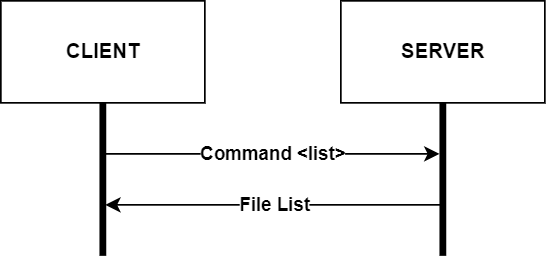
\includegraphics[width=\linewidth]{commandList.png}
  \caption{Schema Comando List}
\end{figure}

\subsubsection{Comando Get}

%%% Comando Get %%%

Il comando \textbf{\emph{get filename}} permette al client di scaricare un file dal server. Il server, dopo aver ricevuto il comando ed il nome del file da scaricare
ne verifica l'esistenza, se il file dovesse essere presente in memoria inizierà la trasmissione con il client per il download (utilizzando un sistema basato sul protocollo rdt 3.0), altrimenti restituirà un messaggio di errore. 

\begin{figure}[!htb]
  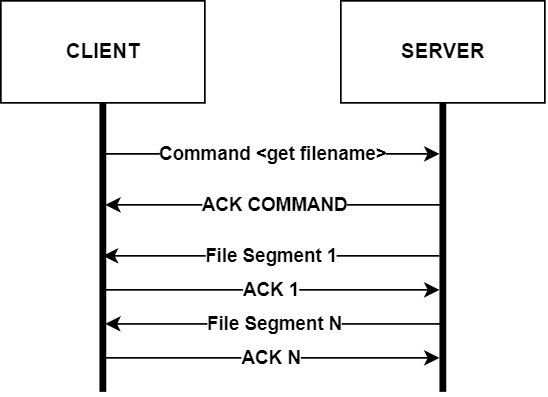
\includegraphics[width=\linewidth]{commandGet.png}
  \caption{Schema Comando Get}
\end{figure}

\subsubsection{Comando Put}

%%% Comando Put %%%

Il comando \textbf{\emph{put filename}} permette al client di caricare un file sul server. Il server, dopo aver ricevuto il comando ed il nome del file da caricare, risponde con un messaggio di ACK,
ed attende l'inizio della trasmissione del file da parte del client, sempre utilizzando un sistema basato sul protocollo rdt 3.0.

\begin{figure}[!htb]
  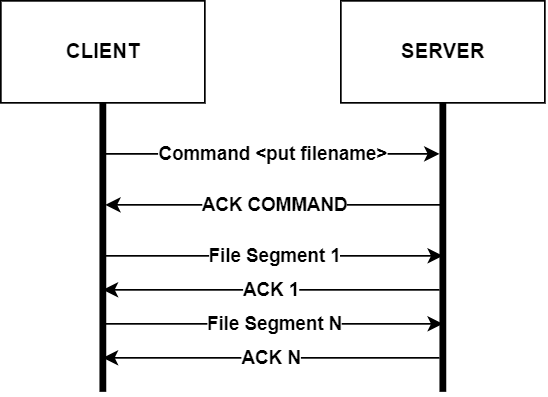
\includegraphics[width=\linewidth]{commandPut.png}
  \caption{Schema Comando Put}
\end{figure}

\newpage
\section{Sviluppo}
\subsection{Client}

%%% Sviluppo Client %%%

La classe Client definisce il socket UDP per la comunicazione con il server.
Tramite un menù di scelta vengono inviati i comandi al server (con il comando  \textit{sendto}) che li gestirà e restituirà il risultato al client.
Ricevuto il risultato dal server (tramite il comando \textit{recvfrom}) eseguirà a seconda del comando inviato:
\begin{itemize}
    \item \textbf{List} stampa nome dei files ricevuti dal server.
    \item \textbf{Put} utilizzo della funzione rdt per la gestione dei pacchetti.
    \item \textbf{Get} controllo l'effettiva esistenza del file e successivamente utilizzo della funzione rdt per la gestione dei pacchetti.
\end{itemize}

\subsection{Server}

%%% Sviluppo Server %%%

Il modulo \textbf{\emph{server.py}} definisce il socket UDP del server attraverso il modulo standard Python: \textbf{\emph{socket.py}}.
Il server, per come è definito, riesce a supportare le richieste di un client alla volta, utilizzando uno switch per smistare i vari comandi (list, get, put).
In caso di richieste di tipo GET e PUT, il server delega la trasmissione o la ricezione dei FILE SEGMENT al modulo \textbf{\emph{rdt\textunderscore handler.py}},
che fornisce i metodi necessari per trasmettere o ricevere file utilizzando il protocollo RDT 3.0.

\subsection{RDT Handler}

Il modulo \textbf{\emph{rdt\textunderscore handler.py}} definisce le strutture dati necessarie per l'implementazione del potocollo RDT 3.0, ed una classe simil controller che espone i metodi per l'interscambio di file utilizzando sempre il protocollo RDT 3.0.\\
Le strutture dati definite da questo modulo sono due: 

	\begin{itemize}
			\item Classe \textbf{\emph{Packet}}: struttura dati principale per l'interscambio dei file segment
			\item Enum \textbf{\emph{PacketType}}: viene utilizzato nella classe Packet e definisce i tipi di pacchetti gestibili (ACK PACKET, DATA PACKET).
		\end{itemize}
	\ \\

La classe \textbf{\emph{RdtFileTransferHandler}} espone i seguenti metodi:

	\begin{itemize}
		\item \textbf{\emph{rdtFileDataReceiver}}: metodo che implementa la logica per la ricezione di un file
		\item \textbf{\emph{rdtFileDataSender}}: metodo che implementa la logica per la trasmissione di un file
	\end{itemize}
\ \\


\newpage
\section{Guida Utente}
\subsection{Client}
Avviato il client comparirà su schermo un menù con le opzioni possibili dei vari comandi.
\subsubsection{Comando List}Per effettuare il comando list basterà selezionare l'apposita opzione dal menù (1), verranno visualizzati i file all'interno della cartella \textit{'upload'}.
\subsubsection{Comando Put}Per effettuare il comando put basterà selezionare l'apposita opzione dal menù (2), verrà chiesto all'utente il nome del file da inserire nella cartella upload, il file dovrà essere presente nella cartella \textit{'ToUpload'} per essere caricato correttamente.
\subsubsection{Comando Get}Per effettuare il comando put basterà selezionare l'apposita opzione dal menù (3), verrà chiesto all'utente il nome del file da scaricare, il file selezionato, in caso sia presente nella cartella 'upload', verrà scaricato nella cartella \textit{'Download'}.
\subsection{Server}

%%% Guida Utente Server %%%

Per avviare il server è sufficiente eseguire il comando:

\begin{verbatim}
python3 server.py
\end{verbatim}

\end{document}